\chapter{Schlussbetrachtungen} % (fold)
\label{cha:schlussbetrachtungen}

In diesem Kapitel werden die Inhalte der gesamten Arbeit zusammengefasst, die Ergebnisse zusammengeführt und einander gegenübergestellt. Ziel dieses Kapitels ist es, letztendlich zu einer Beurteilung der Arbeit hinsichtlich Erfüllung der globalen Zielsetzung zu gelangen. Die Darstellung von weiterem Entwicklungspotential des Werkzeugs schließt die Arbeit ab.

\begin{figure}[htbp]
	\centering
		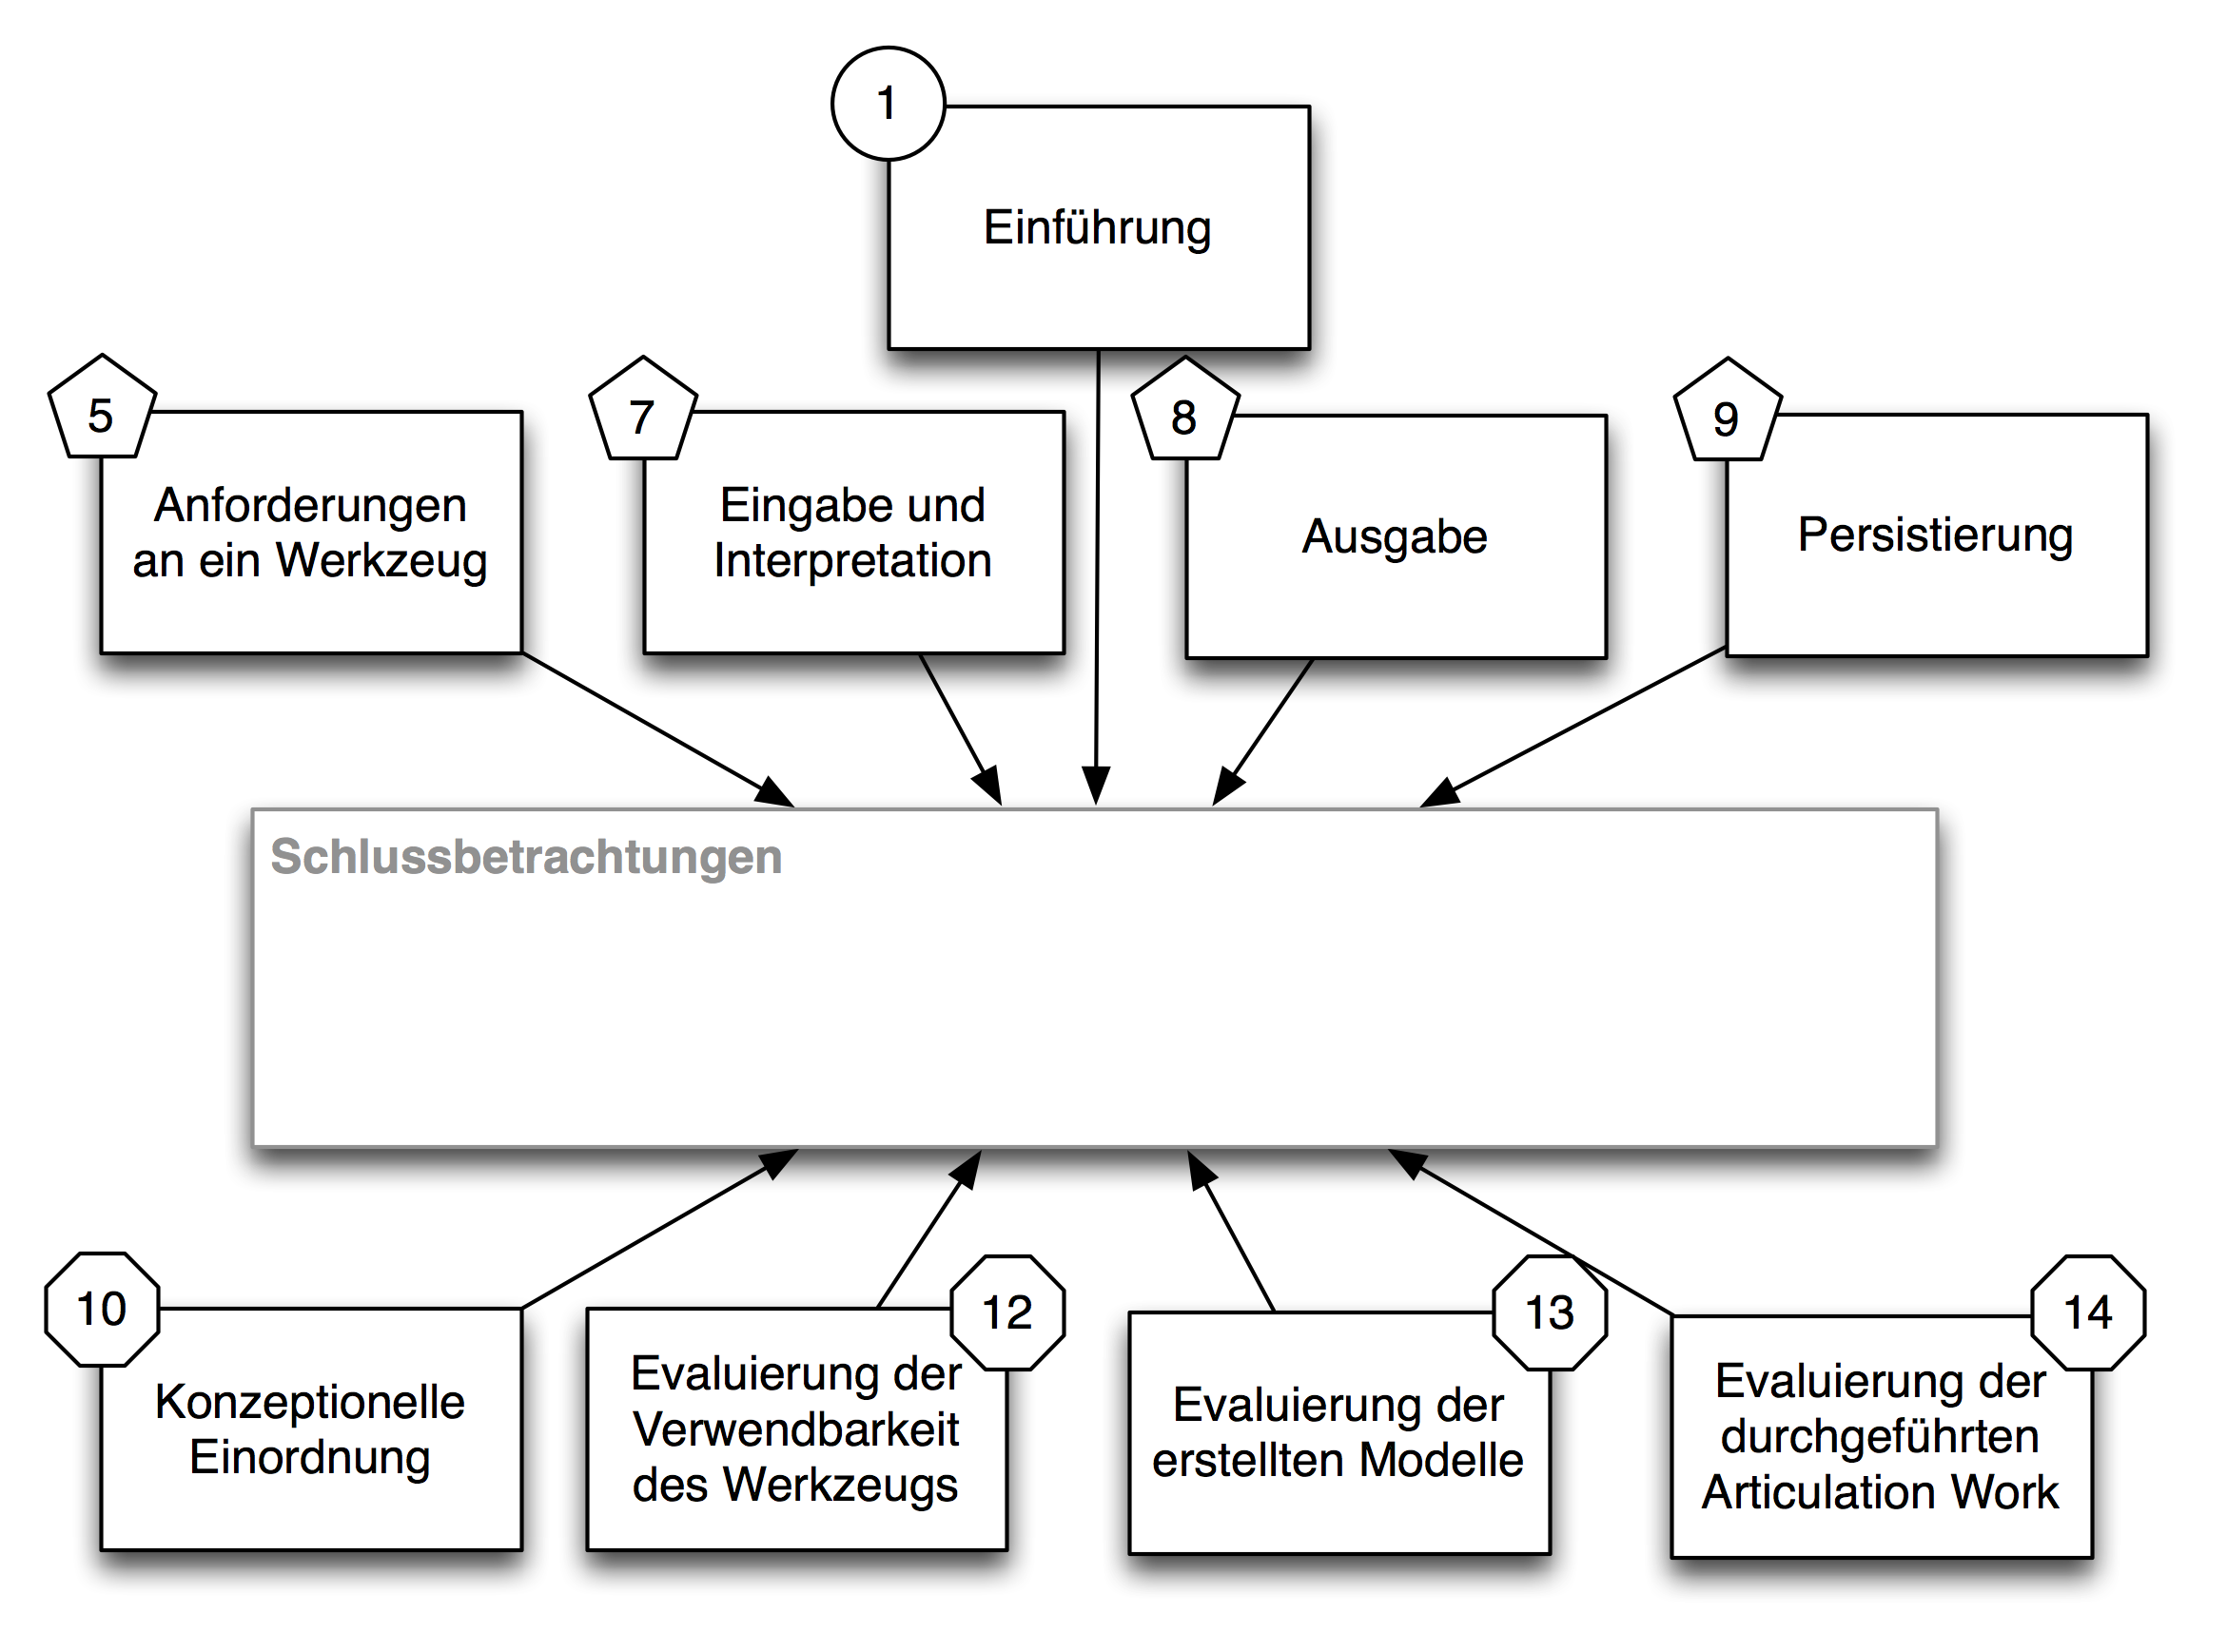
\includegraphics[scale=0.6]{img/Kontextgrafiken/k15.png}
	\caption{Kapitel „Schussbetrachtungen“ im Gesamtzusammenhang}
	\label{fig:img_Kontextgrafiken_k15}
\end{figure}

Abbildung \ref{fig:img_Kontextgrafiken_k15} zeigt die Kapitel, deren Ergebnisse in dieses Kapitel einfließen. Die einzelnen Inhalte werden schrittweise einander strukturiert gegenüber gestellt, was eine Beurteilung der Zielerreichung auf jeder Betrachtungsebene der Arbeit (Fragestellungen der empirischen Untersuchung, Anforderungen an das Werkzeug, Globale Zielsetzung) ermöglicht. Nach einer Darstellung der gesamten dieser Arbeit zugrundeliegenden Konzepte und deren Zusammenhang in der Arbeit in Abschnitt \ref{sec:überblick_über_den_gesamtzusammenhang} werden die einzelnen oben genannten Betrachtungsebenen in umgekehrter Reihenfolge als in der Arbeit dargestellt (also vom Konkreten zum Allgemeinen) einzeln beschrieben. Nach einer Zusammenfassung der Evaluierungsergebnisse und einer Gegenüberstellung mit den Ergebnissen der konzeptuellen Einordnung in Abschnitt \ref{sec:zusammenfassung_der_evaluierung} werden diese in Abschnitt \ref{sec:erfüllung_der_anforderungen_an_das_werkzeug} den in Kapitel \ref{cha:anforderungen} angeführten Anforderungen an das Werkzeug gegenübergestellt. Im letzten Schritt werden die erreichten Ergebnisse hinsichtlich der globalen Zielsetzung bewertet (siehe Abschnitt \ref{sec:bewertung_hinsichtlich_der_globalen_zielsetzung}). Auf Basis dieser Ausführungen ist es in Abschnitt \ref{sec:offene_aspekte_und_entwicklungspotential} möglich, die noch offenen Aspekte dieser Arbeit und weiteres Entwicklungspotential zu identifizieren.

\section{Überblick über die Argumentation in dieser Arbeit} % (fold)
\label{sec:überblick_über_den_gesamtzusammenhang}

In Kapitel \ref{cha:einführung} wurde in Abbildung \ref{fig:img_ArticulationWork_ArbeitInteraktion} die dieser Arbeit zugrunde liegende Konzeptualisierung von Arbeit in „Production Work“ und „Articulation Work“ dargestellt. Auf Basis der Ausführungen in den dazwischen liegenden Kapiteln kann diese Abbildung wie in Abbildung \ref{fig:img_Schlussbetrachtungen_ArbeitInteraktionMentaleModelleTabletop} dargestellt erweitert werden und stellt so die gesamten konzeptuellen Grundbegriffe im Zusammenhang dieser Arbeit dar. Eine detailliertere Betrachtung der Ergebnisse unter Einbeziehung der tatsächlich umgesetzten technischen Unterstützung und den Ergebnissen der empirischen Evaluierung wird in Abschnitt \ref{sec:bewertung_hinsichtlich_der_globalen_zielsetzung} durchgeführt.

\begin{figure}[htbp]
	\centering
	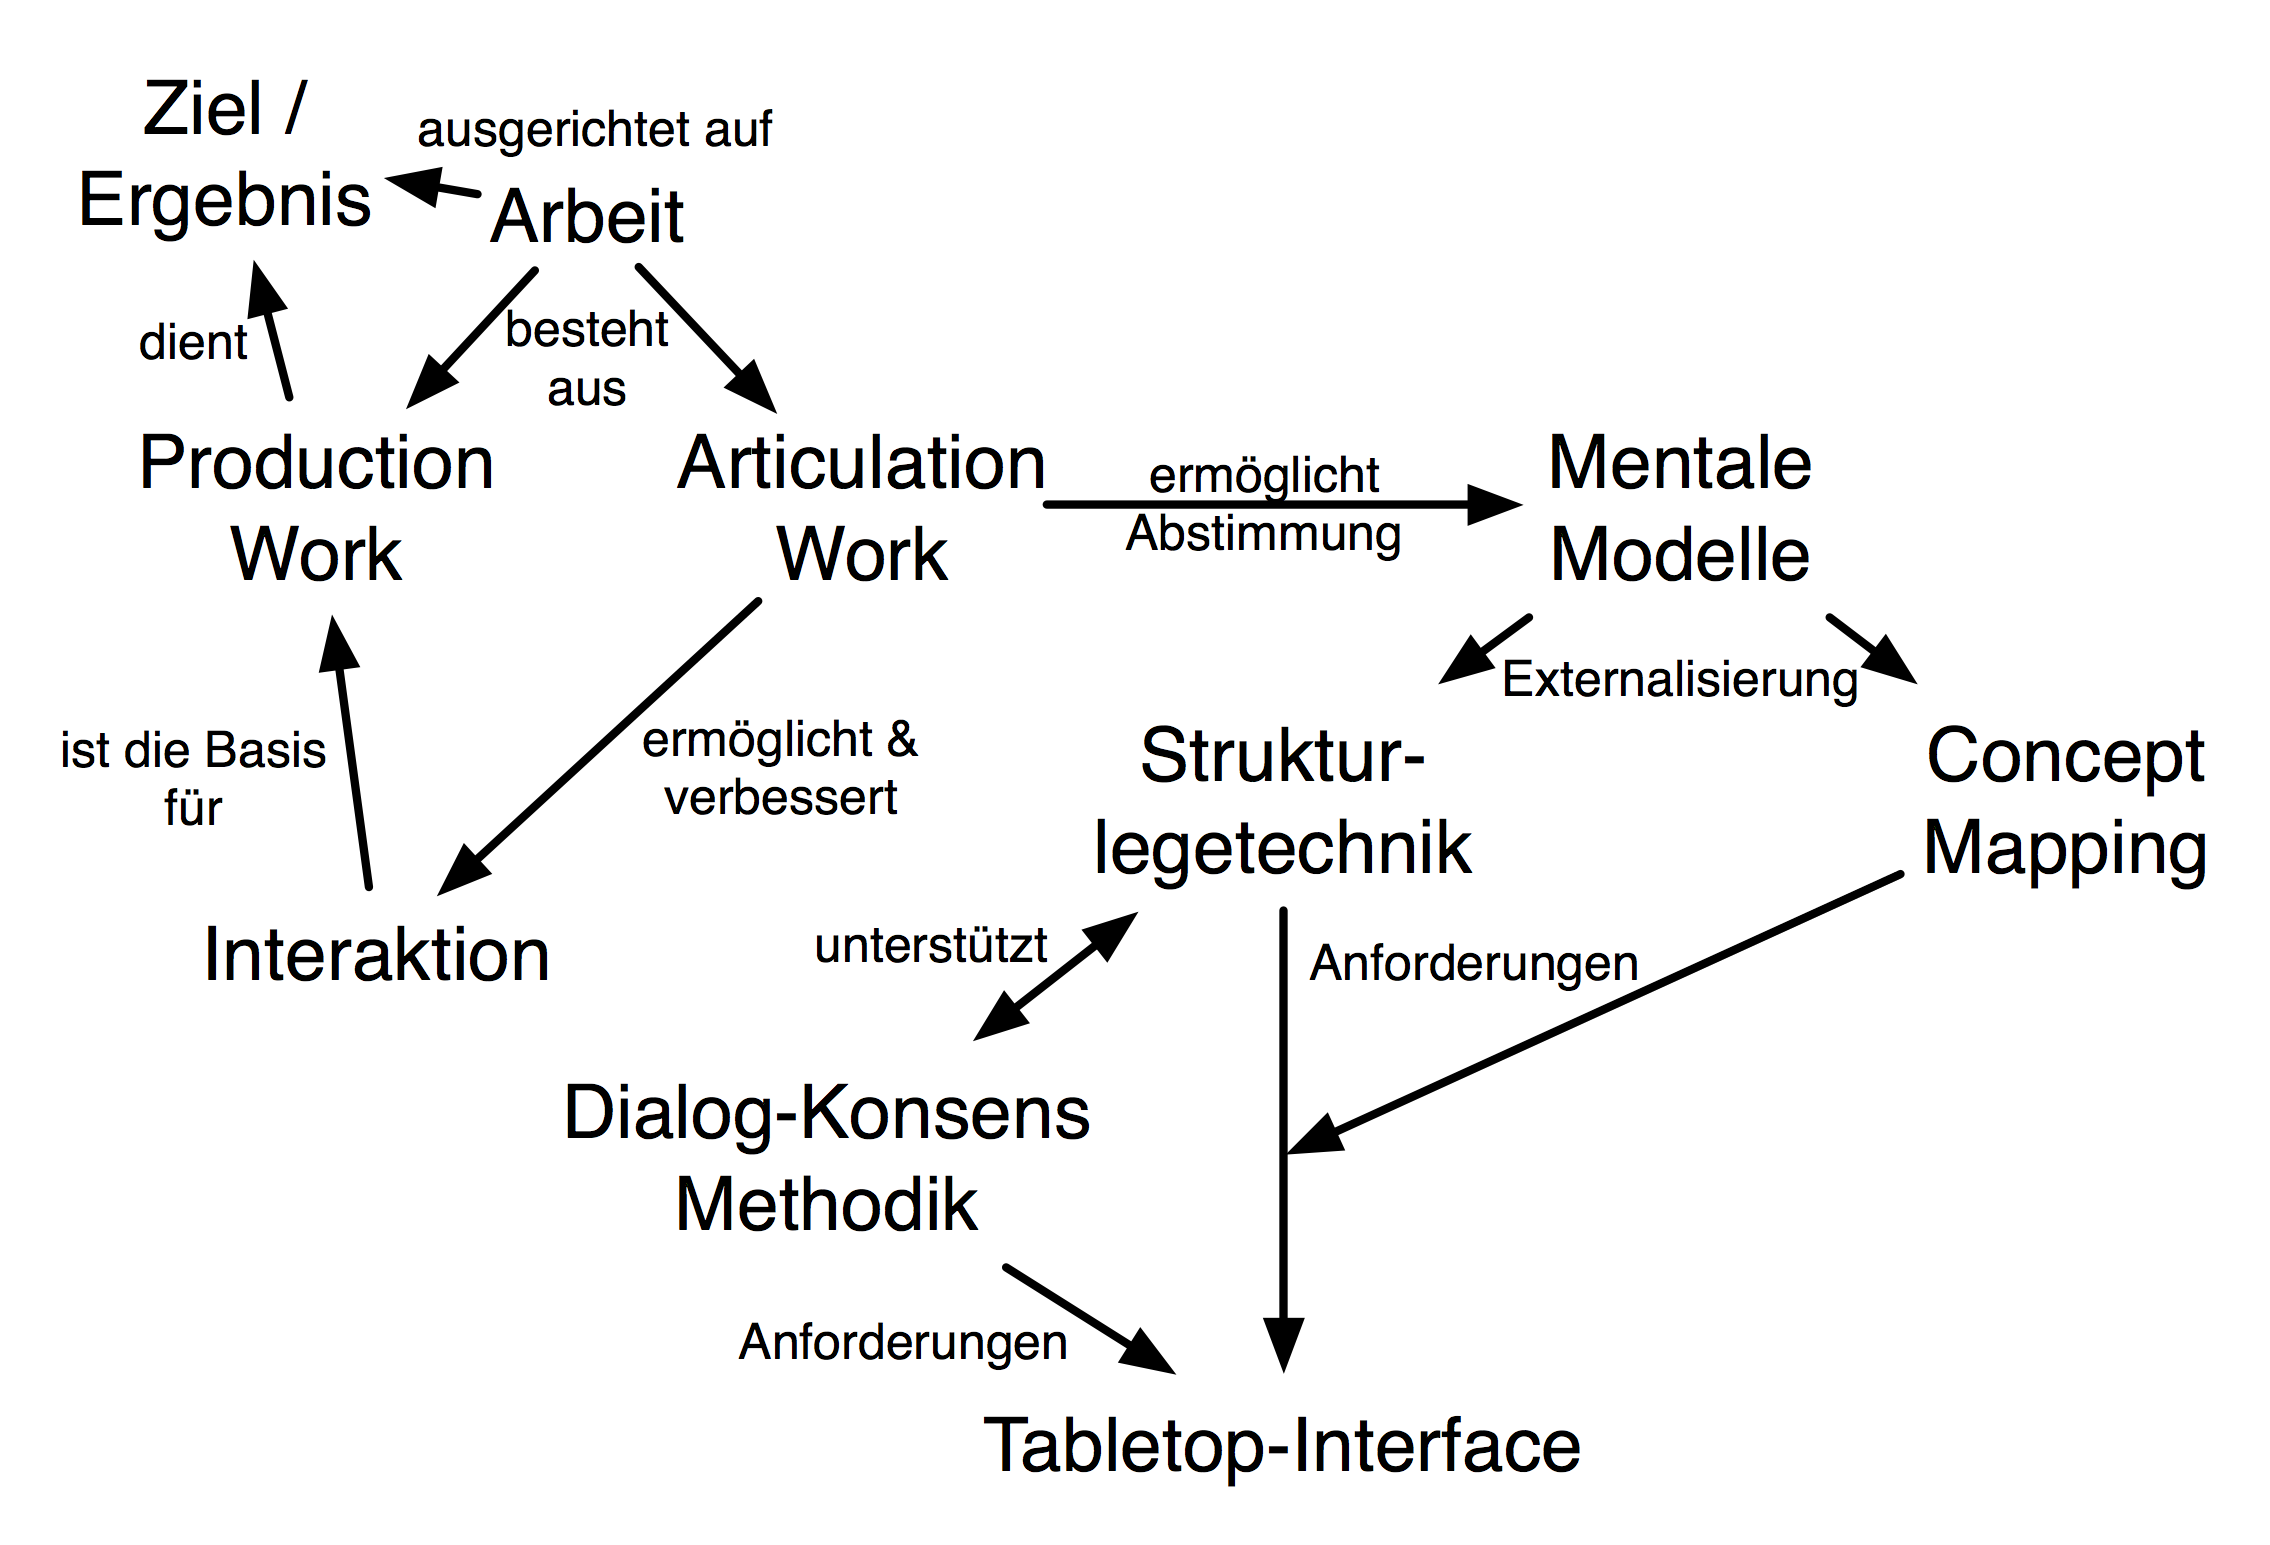
\includegraphics[width=0.9\textwidth]{img/Schlussbetrachtungen/ArbeitInteraktionMentaleModelleTabletop.png}
	\caption{Gesamtzusammenhang der verwendeten Konzepte}
	\label{fig:img_Schlussbetrachtungen_ArbeitInteraktionMentaleModelleTabletop}
\end{figure}

Das Ziel dieser Arbeit ist die Unterstützung der Auflösung von Situationen, in denen produktive Arbeit nicht (mehr) möglich ist. Dies ist dann der Fall, wenn den beteiligten Individuen unklar ist, wie die Zielerreichung gewährleistet werden kann. Diese Arbeit basiert auf der Annahme, dass Interaktion zwischen Individuen immer ein wesentlicher Aspekt bei der Durchführung von Arbeit ist. Arbeit enthält deshalb auch immer Aktivitäten, die mit der Herstellung und Aufrechterhaltung der Interaktion der beteiligten bzw. betroffenen Individuen beschäftigt sind. Dieser Arbeitsanteil wird als „Articulation Work“ bezeichnet. 

Jedes beteiligte Individuum entwickelt auf Basis früherer Erfahrungen oder Lernprozessen Erklärungsmodelle (oder „Mentale Modelle“) für adäquate Aktivitäten bzw. Reaktionen im betreffenden Arbeitsablauf. Wesentlich für die erfolgreiche Interaktion mehrerer Individuen in einem Arbeitsablauf ist die Abstimmung dieser Erklärungsmodelle und die Entwicklung einer gemeinsamen Sichtweise auf jenen Teil des Arbeitsablaufs, in dem zusammengearbeitet werden muss. Diese Abstimmungsprozesse laufen unbewusst immer ab, wenn Individuen interagieren. In bestimmten, als komplex oder problematisch wahrgenommenen Arbeitssituationen reicht die implizite Abstimmung nicht mehr aus -- es ist notwendig, „Articulation Work“ explizit anzustoßen und den Abstimmungsvorgang bewusst zu unterstützen. 

Ein wesentlicher Schritt zur Abstimmung mentaler Modelle ist deren Externalisierung, also deren Abbildung in einer kommunizierbaren Form. Dazu werden unterschiedliche Methoden vorgeschlagen, denen gemein ist, dass die Abbildung in Form diagrammatischer Modelle erfolgt. In der konkreten Umsetzung unterscheiden sich die beiden hier betrachteten Methoden „Strukturlegetechnik“ und „Concept Mapping“ voneinander, bieten aber beide Vorteile bei der Unterstützung der für „Articulation Work“ wichtigen Kommunizierbarkeit mentaler Modelle. In dieser Arbeit werden deshalb diese beiden Ansätze in einer Methodik zusammengeführt, die an die im Rahmen von Strukturlegetechniken vorgeschlagene „Dialog-Konsens-Methodik“ angelehnt ist, in der konkreten Ausführung aber eher der in Concept Mapping vorgeschlagenen Offenheit sowohl des Inhalts als auch der Ausgestaltung des Vorgehens folgt. 

Generell hat bei der Konzeption der Werkzeugunterstützung der bei Strukturlegetechniken vorgeschlagene Ansatz das Primat, weil in ihm die kooperative Durchführung der Modellbildung explizit vorgesehen ist, was der Abstimmung mentaler Modelle eher entgegenkommt als der grundsätzlich eher individuell orientierte Concept-Mapping-Ansatz. Letztendlich wird also in dieser Arbeit der durch Strukturlegetechniken vorgeschlagene Ansatz des physischen, kooperativen Abbildung von Modellen verfolgt, weshalb die Abbildung der Modelle im physischen Raum, konkret auf eine kooperativ bearbeitbaren Tischoberfläche erfolgt. Die Berücksichtigung der Anforderungen des Concept Mapping begründet letztendlich die Notwendigkeit der Hinterlegung der physischen Modellierungsmöglichkeit mit computergestützten Werkzeugen. Um den Anspruch der physischen, kooperativen Modellbildung mit den computergestützten Unterstützungswerkzeugen zu vereinen, wird zur technologischen Umsetzung des Werkzeugs ein „Tabletop Interface“ verwendet, in dem beide Aspekte berücksichtigt und verknüpft werden können.

% section überblick_über_den_gesamtzusammenhang (end)

\section{Zusammenfassung der Evaluierung}
\label{sec:zusammenfassung_der_evaluierung}

In diesem Abschnitt wird die in den Kapiteln \ref{cha:eval_ueberblick}, \ref{cha:eval_werkzeug}, \ref{cha:eval_modell} und \ref{cha:eval_aw} beschriebene empirische Untersuchung zusammengefasst und den Ergebnissen der konzeptuellen Einordnung in Kapitel \ref{cha:konzeptuelle_evaluierung} gegenübergestellt.

\subsection{Empirische Untersuchung}

In der empirischen Untersuchung waren folgende in Kapitel \ref{cha:eval_ueberblick} formulierte Untersuchungsfragen zu beantworten:

\begin{itemize}
 \item Sind das Werkzeug und dessen Komponenten verständlich und wie intendiert einsetzbar? (Untersuchungsgegenstand: Verwendbarkeit des Instruments)
 \item Unterstützt das Instrument die koopertative Modellbildung? (Untersuchungsgegenstand: Kooperative Modellbildung)
 \item Unterstützt das Instrument Articulation Work? (Untersuchungsgegenstand: Wirkung der Articulation Work)
\end{itemize}

Jede dieser Fragen wurde in einem separaten Kapitel bearbeitet. Die Untersuchungsfragen wurden in Hypothesen konkretisiert, die den jeweiligen Untersuchungsgegenstand in Bezug zu den aus den konzeptuellen Grundlagen abgeleiteten Anforderungen an die Unterstützung von „Articulation Work“ stellen.

\paragraph{Verwendbarkeit des Instruments} % (fold)
Bei der Betrachtung der ersten Untersuchungsfrage wurden 8 Hypothesen geprüft, die die grundlegenden Anforderungen an das Werkzeug abdecken bzw. die Verständlichkeit und Verwendbarkeit der implementierten Funktionen testen. Insgesamt scheint das Werkzeug für den intendierten Verwendungszweck -- der kooperativen Erstellung von diagrammatischen Modellen -- in unterschiedlichen Anwendungsgebieten einsetzbar zu sein. Stabilitätsprobleme in der technischen Umsetzung führten in den ersten Phasen der Evaluierung zu Behinderungen bei der Modellbildung, was jedoch durch nachträglich durchgeführte Verbesserungen weitgehend kompensiert werden konnte. Herausforderungen zeigten sich im Interaktionsdesign der über die Kernfunktionalität hinausgehenden Funktionen zur Unterstützung des Modellbildungsprozesses. Die aus der Literatur begründbare Funktion zur Verfolgung der Modellierungshistorie und der Wiederherstellung vergangener Modellzustände wurde kaum genutzt. Auch die Verwendung der Funktion zur Entfernung von unerwünschten Verbindern im Modell war den Benutzern in der ersten Version unverständlich. Dieses Problem konnte durch ein Redesign des entsprechenden Teilwerkzeugs und dessen Bedienung beseitigt werden. Generell scheint das Werkzeug schnell erlernbar zu sein, so dass die Anzahl der Fehlbedienungen durch Missverständnisse bereits bei der zweiten Anwendung des Werkzeugs durch die Benutzer massiv reduziert bzw. nicht mehr vorhanden war. Die oben formulierte Frage kann also mit Vorbehalten positiv beantwortet werden. Generell scheint das Werkzeug wie intendiert einsetzbar und zum Großteil verständlich zu sein, einige Komponenten weisen jedoch Defizite in der Verständlichkeit auf.
% paragraph werkzeug (end)

\paragraph{Kooperative Modellbildung} % (fold)
Für die zweite Untersuchungsfrage wurden 5 Hypothesen geprüft, die sich auf die Verwendung der Werkzeugs zur Modellbildung im Sinne der vorgeschlagenen Methodik zur Unterstützung von „Articulation Work“ beziehen. Insgesamt scheint das Werkzeug zwar nur eingeschränkt für die allgemeine Abbildung von Modellen beliebigen Inhalts und beliebiger Semantik geeignet zu sein. Seinem Verwendungszweck für die auf Modellen basierende Kommunikation und Abstimmung von individuellen Sichtweise scheint das Werkzeug aber zu genügen. Die eingeschränkte Eignung für die Abbildung beliebiger Modelle scheint vor allem in der beschränkten Größe der Modellierungsoberfläche begründet zu liegen, für die die Möglichkeit zur Einbettung von Teilmodellen keinen adäquaten Ersatz darzustellen scheint. Zudem scheint in Einzelfällen die in der aktuellen Hardware-Implementierung vorhandene Beschränkung auf drei semantisch unterschiedliche Modellelementtypen einschränkend wahrgenommen zu werden, was ebenfalls dem Anspruch eines semantisch vollständig offen Modellierungswerkzeugs widerspricht. Dies ist insofern zu relativieren, als dass die Anzahl der Elementtypen in den meisten Fällen zur Kommunikation der individuellen Sichtweisen auszureichen scheint und lediglich in Fällen zu gering wahrgenommen wird, wo eine „vollständige“ Abbildung eines Sachverhaltes angestrebt wurde. Generell scheint das Werkzeug deshalb bei der Modellierung für den intendierten Verwendungszweck in einem Großteil der Anwendungsfälle geeignet zu sein.
% paragraph modell (end)

\paragraph{Wirkung der Articulation Work} % (fold)
In der dritten Untersuchungsfrage wurde letztendlich geprüft, ob das Werkzeug im Sinne der globalen Zielsetzung tatsächlich „Articulation Work“ unterstützt. Dazu wurden 2 Hypothesen gebildet, die die zu erwartenden Wirkungen erfolgreicher „Articulation Work“ abdecken. Die unmittelbare Wirkung der Durchführung von „Articulation Work“ ist die Bildung eines gemeinsamen Verständnisses über den betrachteten Arbeitsgegenstand. Diese Wirkung konnte in der Untersuchung nachgewiesen werden, das Werkzeug erfüllt also diesen Teil der Anforderungen. Mittelbar sollte die Durchführung von „Articulation Work“ auch Auswirkungen auf die betrachteten Arbeitsabläufe selbst haben und die Interaktion im Idealfall verbessern. Derartige Wirkungen konnten jedoch in der Untersuchung nicht nachgewiesen werden. Einige Beobachtungen in Einzelfällen weisen auf eine entsprechende Wirkung hin, insgesamt können diese aber nicht generalisiert werden. Ob die nicht nachweisbare Wirkung am Werkzeug selbst festzumachen ist oder die in der Untersuchung betrachteten Arbeitsabläufe nicht optimal gewählt wurden, wird in weiteren Untersuchung zu prüfen sein.
% paragraph articulation_work (end)

\subsection{Gegenüberstellung der empirischen und konzeptuellen Untersuchung}
\label{sub:gegenüberstellung}

In diesem Abschnitt werden die Ergebnisse der empirischen Untersuchung den in in Abschnitt \ref{sub:verbesserungspotential_für_das_werkzeug} angeführten Konsequenzen für die Werkzeuggestaltung aus dessen konzeptueller Untersuchung gegenübergestellt.

In Kapitel \ref{cha:konzeptuelle_evaluierung} wurde das Werkzeug im Vorfeld der praktischen Untersuchung in die in Abschnitt \ref{sec:konzeptualisierungen_von_tangible_interfaces} beschriebenen Frameworks zur Beschreibung von Tangible Interfaces eingeordnet. Daraus konnte in jenen Fällen Verbesserungpotetial für das Werkzeug abgeleitet werden, in denen die tatsächliche Umsetzung einer Funktionalität des Werkzeugs nicht mit den konzeptuell begründbaren Designentscheidung übereinstimmte. In diesem Abschnitt wird nun angeführt, in welchen Fällen das Verbesserungpotential, d.h. im Umkehrschluss eine Schwäche der aktuellen Implementierung, in der empirischen Untersuchung bestätigt werden konnte. Die Ergebnisse erlauben eine qualitative Aussage über die Eignung der betrachteten Frameworks für die Konzeption von Tangible Interfaces.

\subsubsection{Missverständlichkeit des Löschtokens}

Die ursprüngliche Konzeption des Löschtokens zeigte eine Diskrepanz zwischen dessen wahrgenommener Verwendung und dem tatsächlichen Vorgehen bei dessen Einsatz. Diese Schwäche konnte aus mehreren Frameworks abgeleitet werden, da bei konsistenter Anwendung derselben das Interaktionsdesign anders als tatsächlich umgesetzt hätte ausfallen müssen.

Tatsächlich konnte die Mißverständlichkeit der Löschtokens in der empirischen Untersuchung bestätigt werden (siehe Abschnitt \ref{sub:verwendung_des_löschtokens}). Nach einem Redesign der Verwendung des Löschtokens unter Berücksichtigung der konzeptuell indizierten Gestaltungs-Kriterien traten keine Mißverständnisse mehr auf, das Ausmaß des Einsatzes stieg signifikant an.


\subsubsection{Schwache Ein-Ausgabe-Kopplung bei der Modellierungshistorie}

Nach der Aktivierung der Modellierungshistorie wird diese ausschließlich durch ein Werkzeug auf der Modellierungsoberfläche kontrolliert. Die Ausgabe erfolgt jedoch ausschließlich auf dem sekundären Ausgabekanal, auf der Tischoberfläche erfolgt kein visuelles Feedback weder über die Aktivierung des Historienmodus noch über deren aktuellen Zustand (konkret die aktuelle Position in der Zeitlinie). Nach \citet{Ullmer00} wäre diese schwache Kopplung zu hinterfragen.

In der empirischen Untersuchung konnte dieser Aspekt nicht als Schwachstelle bestätigt werden. Die Entkopplung von Kontrolle und Ausgabe in diesem Anwendungsfall wurde von keinem Teilnehmer als missverständlich wahrgenommen und führte auch nie zu Fehlbedienungen. Dies mag daran liegen, dass der sekundäre Ausgabekanal räumlich nahe an der Tischoberfläche angeordnet war und von vielen Teilnehmern bei der Modellerstellung ohnehin als primäre Informationsquelle -- noch vor der Tischoberfläche selbst -- genutzt wurde. Erst bei der Diskussion verlagerte sich der Fokus der Aufmerksamkeit hin zu dem auf der Tischoberfläche gelegten Modell. Die von der herkömlichen Interaktionsform mit Maus und Tastatur vertraute entkoppelte Ein- und Ausgabe scheint in diesem Fall Bedienungsprobleme vermieden zu haben. Dass keine Desorientierung der Benutzer beim Wechsel in den Historienmodus auftrat, scheint damit zu begründen sein, dass der sekundäre Ausgabekanal permanent aktiv war, den Modellzustand immer synchron darstellte und deshalb wie oben erwähnt oft ohnehin als primärer Informationskanal genutzt wurde.  

\subsubsection{Lange Antwortzeiten auf Interaktionen}

In der ersten Implementierung des Systems kam es vor allem bei der Interaktion zur Herstellung von Verbindern zu Verzögerungen in der Reaktion des Systems. Diese Verzögerungen sollten nach \citet{Bellotti02} vermieden werden, um den Benutzern adäquat Rückmeldung über deren Interaktionswunsch geben zu können.

In der empirischen Untersuchung konnte diese Schwachstelle bestätigt werden. Die Möglichkeit zur Herstellung von Verbindern wurde in der ursprünglichen Implementierung kaum genutzt. Erst als eine weitere Möglichkeit zur Herstellung von Verbindern implementiert wurde, deren wahrgenommener Reaktionszeit geringer war, wurde diese Möglichkeit in signifikant höherem Ausmaß genutzt (siehe Abschnitt \ref{sub:herstellung_von_verbindern}).

\subsubsection{Fehlende einfache Undo-Funktion}

Die Möglichkeit zur Wiederherstellung von vergangenen Modellzuständen ("Undo") ist in der aktuellen Implementierung zwar gegeben, bedingt aber eine zeitaufwändige und in mehreren Schritten durchzuführende Interaktion mit dem System. Dies sollte nach \citet{Bellotti02} vermieden werden, auch das Schema von \citet{Shaer04} lässt hier Inkonsistenzen mit den den ansonsten ausschließlich in einem Bedienungsschritt ausführbaren Interaktionen mit dem Werkzeug erkennen.

In der empirischen Untersuchung wurde die Möglichkeit zur Wiederherstellung zwar verwendet, das Ausmaß des Einsatzes sank aber signifikant, als das Löschtoken neu gestaltet wurde und so eine einschrittige Interaktion zur Korrektur von fehlerhaften Verbindungen (dem häufigsten Grund des Einsatz der Undo-Funktion) geschaffen wurde. Die Gestaltung der Wiederherstellungsfunktion kann damit als Schwachstelle bestätigt werden.

\subsubsection{Mangelnde Verständlichkeit des Snapshot-Tokens}

Das Design des Snapshot-Tokens weist in der derzeitigen Umsetzung nicht auf dessen Funktion hin, was nach bei einer Einordnung in die Taxonomie nach \citet{Fishkin04} gegenüber den anderen Werkzeugen inkonsistent ist. Das Token suggeriert zwar nicht wie im Fall des Löschtoken eine andere Funktionalität, gibt aber den Benutzern durch sein Erscheinungsbild keinen Hinweis auf die Verwendung (mangelhafte Affordances \citep{Norman90}).

Tatsächlich zeigt sich in der empirischen Untersuchung, dass die Funktion zur expliziten Erfassung von Snapshots kaum bzw. in den meisten Anwendungen nicht verwendet wird. Trotz einer erklärenden Einführung in das Werkzeug vor der Modellbildung bestehen häufig Unklarheiten zur Verwendung des Tokens, sobald Benutzer während der Anwendung damit konfrontiert werden. Auch diese Designentscheidung ist damit als Schwachstelle zu bestätigen. 

\subsubsection{Funktional belegte Bereich der Modellierungsoberfläche}

Der hier beschriebene Aspekt ist keine Schwachstelle des Werkzeugs sondern eine Erweiterungsmöglichkeit, die auf Basis der Ausführungen von \citet{Ishii97} identifiziert wurde. Die Autoren schlagen vor, Teile der Interaktionsoberfläche („Trays“) mit Funktionen zu belegen, die eine bestimmte Operation auf einem auf ihm platzierten Token ausführen (etwa: „Details anzeigen“). Bei der Umsetzung des Werkzeugs wurde diese Möglichkeit nicht berücksichtigt, es sind jedoch sinnvolle Anwendungsmöglichkeiten denkbar.

In der empirischen Untersuchung wurden derartige Funktionen von keinen Benutzern erwartet oder gefordert. Da diese Form der Interaktion aber nicht der gängigen Desktop-Metapher entspricht, ist dies auch nur eingeschränkt zu erwarten. Es kann damit auf Basis der Untersuchung keine Aussage über die Notwendigkeit oder Sinnhaftigkeit einer derartigen Erweiterung getroffen werden.

\subsubsection{Verwendbarkeit frei wählbarer Tokens}

Zur Anpassung des Modellierungswerkzeugs an die jeweilige Anwendungsdomäne führt \citet{Holmquist99} als Möglichkeit die Verwendung von domänenspezifischen Token an. Diese Forderung ist grundsätzlich mit den Ansprüchen der semantischen Offenheit des Werkzeugs und der domänenübergreifenden Anwendbarkeit des Ansatzes vereinbar und stützt diese. In der derzeitigen Implementierung ist die Zahl der unterschiedlichen Modellelementtypen auf drei begrenzt. Diese Elementtypen sind in generischen Formen ausgeführt und per se nicht intuitiv domänenspezifisch interpretierbar.

In der empirischen Untersuchung wurde mehrfach die Forderung nach einer höheren Anzahl von unterschiedlichen Elementtypen geäußert, was aber die hier betrachtete Erweiterungsmöglichkeit nur am Rande betrifft (die Verwendung beliebiger Elementtypen würde deren Anzahl zwar erhöhen, umgekehrt implizit die Forderung nach mehr Elementtypen nicht jene nach beliebigen Ausprägungen derselben). Tatsächlich wurde aber in einigen Anwendungen explizit der Wunsch geäußert, Objekt aus dem spezifischen Anwendungsfall (etwa Dokumente oder Werkzeuge) als Tokens verwenden zu können. Dies entspricht im Wesentlichen der oben beschriebenen Erweiterungsmöglichkeit, weshalb diese als sinnvoll erachtet werden kann. 

\subsubsection{Zusammenfassung} % (fold)
\label{ssub:gegenüberstellung_zusammenfassung}

Die in der konzeptuellen Einordnung des Werkzeugs identifizierten Inkonsistenzen im Design und Verbesserungspotentiale konnten in der empirischen Untersuchung großteils bestätigt werden. In jenen Fällen, in denen die konzeptuell identifizierten Lösungsmöglichkeiten in der Praxis umgesetzt wurden, zeigte sich auch jeweils eine Verbesserung der Verständlichkeit bzw. der Bedienbarkeit des Werkzeugs.

Insgesamt erschienen die Ansätze von \citet{Bellotti02}, \citet{Shaer04} und \citet{Fishkin04} als geeignet für den Einsatz im Design von begreifbaren Benutzungsschnittstellen. Während \citet{Bellotti02} allgemeine Richtlinie für die Gestaltung von Benutzungsschnittstellen vorschlägt, ohne konkret auf Tangible Interfaces einzugehen, fokussieren \citet{Shaer04} und \citet{Fishkin04} explizit auf dieses Gebiet. Dabei scheint  sich die Arbeit von \citet{Shaer04} insbesondere für die Gestaltung der Interaktionsabläufe an der Benutzungsschnittstelle und deren konkrete Werkzeugunterstützung zu eignen. Die Arbeit von \citet{Fishkin04} erlaubt hingegegen die Beurteilung der Konsistenz der Bedienkonzepte und ermöglicht so die Identifikation von möglicherweise missverständlichen Aspekten bei der Bedienung der Schnittstelle (siehe dazu auch \citep{Oppl09d}).

% subsubsection zusammenfassung (end)

\section{Erfüllung der Anforderungen an das Werkzeug}
\label{sec:erfüllung_der_anforderungen_an_das_werkzeug}

In diesem Abschnitt werden die in Kapitel \ref{cha:anforderungen} formulierten Anforderungen an das Werkzeug hinsichtlich ihrer Erfüllung betrachtet. Die Beurteilung der Erfüllung erfolgt anhand der empirischen Ergebnisse, die in den Kapiteln \ref{cha:eval_werkzeug}, \ref{cha:eval_modell} und \ref{cha:eval_aw} beschrieben wurden.

\subsubsection{Anforderung \ref{anf:physische_abbildung_legen_beliebiger_diagrammatischer_modelle}}
Anforderung \ref{anf:physische_abbildung_legen_beliebiger_diagrammatischer_modelle} („Physische Abbildung beliebiger diagrammatischer Modelle“) wurde in den Hypothesen \ref{hyp:diagmodelle}, \ref{hyp:behinderung} und \ref{hyp:gewöhnung} untersucht. Die grundlegende Abbildung diagrammatischer Modelle mit dem Werkzeug ist ohne Einschränkung der Anwendungsdomäne möglich. Bei der Untersuchung des Prozesses der physischen Abbildung der Modelle konnten in den ersten durchgeführten Evaluierungsblöcken behindernde Aspekte identifiziert werden. Diese hatten Einfluss auf die Abbildung der Modelle, insbesondere die Möglichkeit des Einsatzes von Verbindern im Modell wurde nur eingeschränkt wahrgenommen. 

Nach Überarbeitungen des Interaktionsdesigns und der Implementierung mehrerer Maßnahmen zur Steigerung der Robustheit gegenüber Fehlerkennungen von Benutzereingaben konnten die als behindernd wahrgenommenen Faktoren reduziert werden. Bei mehrmaliger Verwendung des Werkzeugs zeigt sich eine Verbesserung des Umgangs mit den zur Verfügung gestellten Ausdrucksmöglichkeiten und eine stärke Fokussierung auf den zu repräsentierenden Sachverhalt. Insgesamt kann diese Anforderung als erfüllt angesehen werden.

\subsubsection{Anforderung \ref{anf:unterstützung_der_iterativen_aushandlung_des_modells}}
Anforderung \ref{anf:unterstützung_der_iterativen_aushandlung_des_modells} („Unterstützung der iterativen Aushandlung des Modells“) wurde in Hypothese \ref{hyp:abstimmung} untersucht. Ziel der Unterstützung von Aushandlungsprozessen ist die Bildung einer gemeinsamen Sichtweise auf das betrachtete Problem. Die kooperative Modellierung ist durch das Design von Hard- und Software grundsätzlich möglich, durch die Verwendung eines Tabletop Interface wird die kooperative Modellbildung und der Austausch über den Modellierungsgegenstand (also das betrachtete Problem) ermöglicht. Die beabsichtigte Wirkung der Abstimmung der individuellen Sichtweisen konnte in der empirischen Untersuchung bestätigt werden. Insgesamt kann diese Anforderung also bestätigt werden.

\subsubsection{Anforderung \ref{anf:ermöglichung_experimenteller_veränderungen_am_modell}}
Anforderung \ref{anf:ermöglichung_experimenteller_veränderungen_am_modell} („Ermöglichung experimenteller Veränderungen am Modell“) wurde in Hypothese \ref{hyp:wiederherstellung} untersucht. Experimentelle Veränderungen am Modell werden durch die Unterstützung der Wiederherstellung von vergangenen Modellzuständen realisiert. Diese Funktion wurde technisch implementiert und hinsichtlich ihrer Funktionsfähigkeit getestet. Diese ist vollständig gegeben. 

In der empirischen Untersuchung wurde die Funktionalität von den Teilnehmern jedoch nicht genutzt, so dass die Erfüllung der Anforderung empirisch nicht bestätigt werden kann. Aus den Ergebnissen der Untersuchung ist vielmehr zu hinterfragen, ob diese aus der Theorie der Externalisierung mentaler Modelle abgeleitete Anforderung in der Praxis tatsächlich relevant ist.

\subsubsection{Anforderung \ref{anf:nicht_vorgegebene_semantik_der_modellierungselemente}}
Anforderung \ref{anf:nicht_vorgegebene_semantik_der_modellierungselemente} („Nicht vorgegebene Semantik der Modellierungselemente“) wurde in den Hypothesen \ref{hyp:kontexte} und \ref{hyp:keine_einschränkung} untersucht. Durch die nicht vorgegebene Semantik der Modellierungselemente wird einerseits der Einsatz des Werkzeugs in unterschiedlichen Anwendungskontexten ermöglicht, andererseits werden Benutzer nicht gezwungen, ein vorgegebenes Abbildungsschema für die von ihnen auzudrückende Information zu verwenden. Dies ermöglicht ein Fokussierung auf die Modellierungsinhalte und die Kommunikation derselben und vermeidet einen zusätzlichen -- potentiell kognitiv belastenden -- Übersetzungsschritt. Die Wahl der Bedeutung der Modellierungselemente scheint sich aus der ohnehin ablaufenden Interaktion zu ergeben und keine Probleme zu verursachen. 

Technisch wurde diese Anforderung durch die Verwendung generischer (also semantisch nicht vorbelegter) Modellierungsbausteine in Kombination mit dem Einsatz von Topic Maps zur Repräsentation der Modelle umgesetzt. Das Werkzeug erlaubt grundsätzlich die Verwendung von beliebigen und beliebig vielen unterschiedlichen Modellierungsbausteinen, diese Möglichkeit wurde jedoch im vorliegenden Prototypen nicht eingesetzt. 

Die empirische Untersuchung konnte die Einsetzbarkeit in unterschiedlichen Anwendungskontexten ohne Einschränkung bestätigen. Die Modellierung selbst wurde jedoch durch die im Prototypen auf drei unterschiedliche Modellierungselemente eingeschränkte Ausdrucksstärke des Werkzeugs teilweise als einschränkend empfunden. Da dies jedoch keine konzeptuelle Einschränkung ist, sondern ausschließlich dem aktuellen Entwicklungsstand der Werkzeug-Hardware geschuldet ist, kann diese Anforderung insgesamt als erfüllt angesehen werden. 

\subsubsection{Anforderung \ref{anf:verknüpfung_mit_digitalen_ressourcen}}
Die Erfüllung von Anforderung \ref{anf:verknüpfung_mit_digitalen_ressourcen} („Verknüpfung mit digitalen Ressourcen“) wurde im Rahmen der durchgeführten Studien nicht untersucht. Die Verknüpfung mit digitalen Ressourcen wurde analog zur Funktion zur Einbettung von Teilmodellen implementiert. Digitale Dokumente können an einbettbare Tokens gebunden werden und in einem Container durch Hineinlegen zugewiesen werden. Diese Funktionalität wurde technisch implementiert und hinsichtlich ihrer Funktionsfähigkeit getestet. 

Im Rahmen der Evaluierung wurde das Werkzeug ausschließlich mit einem Rechner betrieben, auf dem keine fallspezifischen bzw. anwendungsrelevanten digitalen Dokumente vorhanden waren. Die Einbindung von Dokumenten in Modelle konnte deswegen nicht vorgenommen werden. Die Anforderung ist also technisch erfüllt, konnte jedoch empirisch nicht überprüft werden. 

\subsubsection{Anforderung \ref{anf:bearbeitung_von_beliebig_komplexen_modellen}}
Anforderung \ref{anf:bearbeitung_von_beliebig_komplexen_modellen} („Bearbeitung von beliebig umfangreicher Modellen“) wurde in Hypothese \ref{hyp:beliebige_komplexität} untersucht. Durch die physisch beschränkte Größe der Modellierungsfläche kann die Erweiterung der Modellgröße lediglich durch die Erstellung von Teilmodellen erreicht werden, wobei deren Zusammenhang durch die Einbettung der Teilmodelle in Überblicksmodelle ausgedrückt wird. Die Einbettung von Teilmodellen wird mittels der Verwendung von Modellierungsblöcken als Container realisiert, in die Tokens als Repräsentaten der Teilmodelle gelegt werden können. Die dazu notwendigen Funktionen wurden technisch implementiert und hinsichtlich ihrer Funktionsfähigkeit erfolgreich getestet. 

Auch in der empirischen Untersuchen wurde die Erweiterung der Modellgröße durch Einbettung von Teilmodellen erfolgreich eingesetzt. Im Vergleich der erstellten Modelle mit Modellen, die mit einem Werkzeug mit nicht beschränkter Modellierungsfläche erstellt wurden, zeigte sich jedoch eine signifikant geringere Modellgröße bei der Erstellung mit dem hier vorgestellten System. Die Erstellung beliebig großer Modelle ist somit technisch grundsätzlich möglich und auch verwendbar, empirisch konnte die Erfüllung der Anforderung dennoch nicht nachgewiesen werden.

\subsubsection{Anforderung \ref{anf:kollaborative_und_unmittelbare_manipulierbarkeit_des_modells}}
Anforderung \ref{anf:kollaborative_und_unmittelbare_manipulierbarkeit_des_modells} („Kooperative und unmittelbare Manipulierbarkeit des Modells“) wurde in den Hypothesen \ref{hyp:kollaborativ} und \ref{hyp:stärkere_kooperation} untersucht. Die Möglichkeit, Modelle kooperativ zu erstellen und zu manipulieren, ist grundsätzlich gegeben, die Möglichkeit der Durchführung eines kooperativen Modellierungsprozesses konnte empirisch belegt werden. Im Vergleich zu einem bildschirmbasierten System zeigt sich außerdem ein signifikant höherer Anteil an Interaktion zwischen den Teilnehmern bei der Durchführung der Modellierung mit dem hier vorgestellten System. Die Anforderung kann somit als erfüllt angesehen werden.

\subsubsection{Anforderung \ref{anf:persistente_ablage_des_modells_möglichkeit_zur_rekonstruktion}}
Anforderung \ref{anf:persistente_ablage_des_modells_möglichkeit_zur_rekonstruktion} („Persistente Ablage des Modells und Möglichkeit zur Rekonstruktion“) wurde in Hypothese \ref{hyp:historie} untersucht. Die Persistente Ablage der erstellten Modelle wurde mittels XML-Topic Maps realisiert. Die Funktionsfähigkeit der Persistierung wurde insofern technisch nachgewiesen, als dass die exportierten Modellrepräsentationen valide \gls{XTM}-Dateien waren und sämtliche auf der Modellierungsoberfläche repräsentierte Information in der Datei abgebildet war. 

Hinsichtlich der Ermöglichung der Rekonstruktion und der Nachvollziehbarkeit des Modellierungsprozesses konnte gezeigt werden, dass die bei der Persistierung inkludierte Entstehungshistorie des Modells die Nachvollziehbarkeit der im Modell repräsentierten Information zwar tendenziell erleichterte, aber nicht in allen Fällen ermöglichte. Die Anforderung kann damit technisch als erfüllt angesehen werden, die positive Wirkung der eingebetteten Entstehungshistorie des Modells konnte ebenfalls bestätigt werden. Insgesamt ist die Nachvollziehbarkeit der Modelle ausschließlich auf Basis der gespeicherten Repräsentationen aber in Frage zu stellen.

\subsubsection{Zusammenfassung}
Zusammenfassend ergibt sich hinsichtlich der Erfüllung der Anforderungen die in Tabelle \ref{tab:erfuellung_der_anforderungen} dargestellte Übersicht. In ihr sind die Anforderungen jenen Kapiteln und Abschnitten des Implementierungsteils (\emph{Impl.}) zugewiesen, in denen ihre technische Umsetzung beschrieben wird, sowie den Hypothesen (\emph{Hyp.}) zugeordnet, in denen die tatsächliche Überprüfung der Erfüllung durchgeführt wird.

\begin{table}[htbp]
	\centering
	\caption{Erfüllung der Anforderungen}
\begin{tabular}{| c | p{5cm} | p{1cm} | c | p{4cm} |} 
  \hline
  & Anforderung & Impl. & Hyp. & Beurteilung \\ \hline \hline
  \ref{anf:physische_abbildung_legen_beliebiger_diagrammatischer_modelle} & Physische Abbildung beliebiger diagrammatischer Modelle &  \ref{sub:erkennen_von_verbindungen}, \ref{sub:benennung_von_modellelementen}, \ref{sub:ausgabe_von_information_zum_modell} & \ref{hyp:diagmodelle}, \ref{hyp:behinderung}, \ref{hyp:gewöhnung} & technisch möglich, empirisch teilweise bestätigt \\ \hline
  \ref{anf:unterstützung_der_iterativen_aushandlung_des_modells} & Unterstützung der iterativen Aushandlung des Modells & \ref{ssub:zustands_und_ereignismeldungen} & \ref{hyp:abstimmung} & technisch möglich, empirisch bestätigt \\ \hline
  \ref{anf:ermöglichung_experimenteller_veränderungen_am_modell} & Ermöglichung experimenteller Veränderungen am Modell & \ref{sub:tracking_des_modellzustandes}, \ref{ssub:wiederherstellungsunterstützung} & \ref{hyp:wiederherstellung} & technisch möglich, empirisch nicht bestätigt \\ \hline \hline
  \ref{anf:nicht_vorgegebene_semantik_der_modellierungselemente} & Nicht vorgegebene Semantik der Modellierungselemente & \ref{sub:festlegung_der_bedeutung_von_modellelementen}, \ref{sub:abbildung_des_metamodells} & \ref{hyp:kontexte}, \ref{hyp:keine_einschränkung} & technisch möglich, empirisch teilweise bestätigt \\ \hline
  \ref{anf:verknüpfung_mit_digitalen_ressourcen} & Verknüpfung mit digitalen Ressourcen & \ref{sub:erkennung_von_geöffneten_tokens}, \ref{sub:ausgabe_von_information_zum_modell} & --- & technisch möglich, empirisch nicht geprüft \\ \hline
  \ref{anf:bearbeitung_von_beliebig_komplexen_modellen} & Bearbeitung von beliebig umfangreicher Modellen & \ref{sub:erkennung_von_geöffneten_tokens} & \ref{hyp:beliebige_komplexität} & technisch möglich, empirisch nicht bestätigt \\ \hline \hline
  \ref{anf:kollaborative_und_unmittelbare_manipulierbarkeit_des_modells} & Kooperative und unmittelbare Manipulierbarkeit des Modells & \ref{sub:verteilung_des_modellzustandes}, \ref{sub:einsatz_von_jhotdraw} & \ref{hyp:kollaborativ}, \ref{hyp:stärkere_kooperation} & technisch möglich, empirisch bestätigt \\ \hline
  \ref{anf:persistente_ablage_des_modells_möglichkeit_zur_rekonstruktion} & Persistente Ablage des Modells und Möglichkeit zur Rekonstruktion & \ref{sub:tracking_des_modellzustandes}, \ref{ssub:abruf_der_modellierungshistorie}, \ref{sub:grundlegende_abbildung} & \ref{hyp:historie} & technisch möglich, empirisch bestätigt \\ \hline 
\end{tabular}
	\label{tab:erfuellung_der_anforderungen}
\end{table}


\section{Bewertung hinsichtlich der globalen Zielsetzung}
\label{sec:bewertung_hinsichtlich_der_globalen_zielsetzung}

In diesem Abschnitt wird die Arbeit hinsichtlich der globalen Zielsetzung zusammengefasst, reflektiert und beurteilt. In Kapitel \ref{cha:einführung} wurde die globale Zielsetzung wie folgt formuliert:

\begin{framed}	
	\emph{In der vorliegenden Arbeit sind die Möglichkeiten zur methodischen Unterstützung von expliziter Articulation Work unter Berücksichtigung relevanter Theoriebildungen zur Rolle der beteiligten Individuen zu erfassen, auf Basis dieser Erkenntnisse geeignete Methoden auszuwählen, diese in einem Instrument umzusetzen und dessen Effektivität im Kontext der Production Work zu prüfen.}
\end{framed}


Zur Detaillierung dieser Zielsetzung wurden zwei Forschungsfragen formuliert, die im Folgenden in die Betrachtung einfließen:
\begin{enumerate}
	\item Wie kann die Durchführung und Wirkung von „Articulation Work“ charakterisiert werden?
	\item Wie kann explizite „Articulation Work“ effektiv unterstützt werden?
\end{enumerate}

Bei der Reflexion der Ergebnisse dieser Arbeit hinsichtlich der Forschungsfragen wird jeweils auch auf den Kontext der Arbeit, aus dem die Ableitung der Zielsetzung heraus durchgeführt wurde, Bezug genommen.

\subsection{Wie kann die Durchführung und Wirkung von „Articulation Work“ charakterisiert werden?}

Die globale Zielsetzung stellt den Anspruch, die methodischen  Möglichkeiten der Unterstützung expliziter „Articulation Work“ zu untersuchen. Die Festlegung bzw. Einschränkung auf explizite „Articulation Work“ dient der Abgrenzung der Arbeit zu existierenden Ansätzen, die sozial und/oder technologisch in Arbeitsabläufe intervenieren und dem Auftreten von Unklarheiten vorbeugen bzw. diese durch unmittelbare Unterstützungmaßnahmen auflösen. All diese Ansätze sind in den Bereich der Unterstützung impliziter „Articulation Work“ einzuordnen, die Durchführung derselben ist den handelnden Personen also nicht unbedingt bewusst. 

Treten Situationen auf, die von den Beteiligten als so problematisch wahrgenommen werden, dass eine Aufrechterhaltung des Arbeitsablaufs nicht mehr gewährleistet ist, muss die Handlungsfähigkeit durch explizite Beschäftigung mit der problematischen Situation (wieder) hergestellt werden. Dieser Fall wird als explizite „Articulation Work“ bezeichnet. Das Erfolgskriterium für explizite „Articulation Work“ ist das Erreichen eines Zustandes, in dem gegenseitiges Verständnis soweit (wieder-)hergestellt ist, dass die produktiven Arbeitsabläufe durch implizite „Articulation Work“ aufrecht erhalten werden können. Es müssen somit die methodischen und technischen Voraussetzungen zur erfolgreichen (Wieder-)Erlangung einer gemeinsamen Sichtweise aller Beteiligten auf den als problematisch wahrgenommenen Betrachtungsgegenstand geschaffen werden.

Ein Erklärungsansatz, mit dem das Phänomen von unterschiedlichen Sichtweisen auf den gleichen realen Arbeitsablauf oder -gegenstand erklärt werden kann, sind mentale Modelle. Mentale Modelle beschreiben, wie Individuen aus wahrgenommenen Situationen Handlungsalternativen ableiten und sich letztendlich für die Durchführung bestimmter Aktivitäten entscheiden. Bei kooperativen Arbeitsprozessen ist es notwendig, dass von den Individuen zumindest eine gemeinsame Sichtweise auf die Schnittstellen, an denen diese kooperieren, erreicht wird -- die individuellen mentalen Modelle über diese Schnittstellen müssen also abgestimmt werden. Diese Abstimmung ist eine Ausprägung der Durchführung expliziter „Articulation Work“ -- auch hier gilt, dass nicht sämtliche mentalen Modelle, die den jeweiligen Arbeitsablauf betreffen, abgestimmt werden müssen. Es ist vielmehr ausreichend, lediglich jene Aspekte abzustimmen, die für die Kooperation untereinander relevant sind.

Zur Abstimmung mentaler Modelle ist deren Kommunizierbarkeit eine notwendige Vorbedingung. Diese Kommunizierbarkeit wird durch Externalisierung der mentalen Modelle ermöglicht. Als vorteilhaft für die Kommunikation komplexer Sachverhalte wird in der Literatur die Repräsentation derselben in der Form von diagrammatischen Modellen bezeichnet. Während zur Repräsentation diagrammatischer Modelle grundsätzlich unterschiedliche Möglichkeiten bestehen, werden Strukturlegetechniken und Concept Mapping im Bereich der Externalisierung mentaler Modelle grundsätzlich als geeignet bezeichnet. 

\subsection{Wie kann explizite „Articulation Work“ effektiv unterstützt werden?}

Im Kontext des Einsatzes zur Abstimmung mentaler Modelle sind besonders Strukturlegetechniken als relevant zu betrachten. Deren methodische Hinterlegung durch die Dialog-Konsens-Methodik zielt explizit auf die Bildung eines gemeinsamen Verständnisses ab und eignet sich deshalb für die Unterstützung expliziter „Articulation Work“. In Einzelaspekten, etwa der semantischen Offenheit der Modellierungselemente, bringt aber auch der Ansatz der Concept Maps Konzepte ein, die im Kontext der Durchführung expliziter „Articulation Work“ relevant erscheinen. In dieser Arbeit wird deshalb versucht, eine Variante von Strukturlegetechniken zu entwickeln, die die für „Articulation Work“ relevanten Aspekte von Concept Mapping berücksichtigt und so die Abstimmung mentaler Modelle aus beliebigen Arbeitskontexten ermöglicht. 

Die in dieser Arbeit vorgeschlagene Methodik, die auf den Ansätzen von Strukturlegetechniken und Concept Mapping basiert, bedingt eine Unterstützung durch ein Werkzeug, dass die Abbildung der dazu notwendigen diagrammatischen Modelle unterstützt. Die aus der Methodik abgeleiteten Anforderungen implizieren, dass die Modellierung selbst im physischen Raum durchgeführt wird, diese aber dennoch durch rechnerbasierte Funktionen unterstützt und ergänzt wird. Die Zusammenführung der physischen und digitalen Repräsentation und Interaktonsmechanismen wird durch ein Tangible Tabletop Interface realisiert.

Dieses Werkzeug ermöglicht es, auf einer Tischoberfläche mit physischen Elementen (Bausteinen) diagrammatische Modelle zu erstellen. Die Bausteine werden dazu auf der Tischoberfläche platziert und mittels unterschiedlicher Interaktionen mit dem System untereinander in Beziehung gesetzt. Die Darstellung der Beziehungen erfolgt dabei durch Projektion auf die Tischoberfläche, um eine einfache Manipulierbarkeit des Modells gewährleisten zu können. Um dem Anspruch der semantischen Offenheit des Modells und damit der Anpassbarkeit der Modelle an die individuellen Sichtweisen der Teilnehmer gewährleisten zu können, werden die Modellelemente semantisch nicht vorbelegt, sondern während der Modellbildung durch die Teilnehmer spezifiziert. 

Die Gesamtheit der abgebildeten Modelle inklusive der Festlegung der Bedeutung der Modellelemente wird als semantisches Netzwerk in Form einer Topic Map digital repräsentiert. Dies gewährleistet die Nachvollziehbarkeit und Weiterverwendbarkeit der Modelle auch über einzelne Anwendungen des Werkzeugs hinweg. Zur Unterstützung des Modellierungs- und Abstimmungsprozesses wurden Funktionen entwickelt, die vor allem die einfache und konsequenzlose Veränderbarkeit des Modells gewährleisten sollen. Dazu zählen unter anderem die Verfolgung des Modellierungsprozesses durch das System, die Erfassung stabiler Modellzustände und die Möglichkeit, durch die Entstehungshistorie des Modells zu navigieren und vergangene Modellzustände wieder herzustellen.  

Konkret wurde das Werkzeug hardwareseitig als Tisch mit transparenter Oberfläche ausgeführt. Die Modellierungsoberfläche ist 80 x 100 cm groß und erlaubt die gleichzeitige Verwendung von etwa 15 Modellierungselementen. Die Modellierungselemente sind in drei unterschiedlichen Formen und Farben in Acrylglas ausgeführt und können geöffnet werden. Diese Funktion als Container ermöglicht die Einbettung von zusätzlicher Information in das Modell durch Hineinlegen kleiner informationstragender Elemente. Auch die Einbettung von Teilmodellen und damit einhergehend die Erweiterung der Modellgröße ist möglich. 

Unter der Tischoberfläche ist ein Videoprojektor angebracht, die die Verbindungen im Modell, die Benennung der Modellelemente sowie zusätzliche Information zur Modellierungsunterstützung auf die Oberfläche projiziert. Zusätzlich ist eine zweite Ausgabeoberfläche in Form eines Bildschirms (oder alternativ einer Leinwand mit Projektor) vorhanden, auf der der aktuelle Modellzustand synchron mitgeführt wird und auf dem nicht kohärent auf der Tischoberfläche darstellbare Information, wie etwa die Modellierungshistorie, dargestellt wird. Sämtliche Interaktion mit dem System wird über die Tischoberfläche durchgeführt, lediglich die Benennung der Modellelemente erfolgt alternativ mittels Tastatur, da der auf Bilderkennung basierende primäre Benennungsmechanismus nicht ausreichend stabil für eine komfortable Bedienung arbeitete.

Das Werkzeug kann von mehreren Personen simultan bedient werden und erfasst den Modellierungsverlauf selbständig im Hintergrund. Dies wird einerseits genutzt werden, um Modellvarianten zu erproben und einfach zu einem stabilen, akzeptierten Zustand zurückzukehren und bietet andererseits die Möglichkeit, die gesamte Historie der Modellentstehung persistent abzulegen und zu einem späteren Zeitpunkt wieder abzurufen. In beiden Fällen bietet das Werkzeug Unterstützung bei der Wiederherstellung eines gespeicherten Modellzustandes, indem schrittweise Anweisungen zur Platzierung der entsprechenden Modellelemente auf die Tischoberfläche projiziert werden.

Das Werkzeug wurde in mehreren Revisionen technisch stabilisiert und ermöglicht in seinem derzeitigen Zustand die Durchführung beliebig umfangreicher Modellbildungen mit beliebiger zeitlicher Ausdehnung. Die Softwarekomponenten sind außerdem für eine etwaige Kopplung mehrerer physischer oder digitaler Modellbildungs-Werkzeugs (etwa weiterer Modellierungtische) vorbereitet, um auch räumlich entfernte Kooperation zu ermöglichen. 

Die Untersuchung der effektiven Unterstützung von explizter Articulation Work bedingt die Konkretisierung des Effektivitäts-Begriff. Grundsätzlich wird Articulation Work immer im Zusammenhang mit einem konkreten Arbeitsprozess (der Production Work) bzw. mit einer in diesem aufgretretenen problematischen Situation durchgeführt. Die Wirkung von Articulation Work zeigt sich an damit unmittelbar an der Production Work und an den in diesem beteiligten Individuen. Articualtion Work ist dann effektiv, wenn die beteiligten Personen die Situation nicht mehr als problematisch wahrnehmen  und die Production Work (wieder) ohne Hindernisse durchgeführt werden kann. Eine Voraussetzung zur Durchführung effektiver expliziter Articulation Work ist aus methodischer Sicht die Durchführung der kooperativen Modellbildung, die zur Abstimmung der individuellen mentalen Modelle über die Production Work verwendet wird. Hinsichtlich der koopertiven Modellbildung ist als Voraussetzung der effektiven Unterstützung expliziter Articulation Work die Fähigkeit des Instruments zu sehen, die zur Durchführung der Modellbildung notwendigen Schritte für die beteiligten Individuen verständlich und benutzbar zu unterstützen.

Hinsichtlich des letztgenannten Aspektes wurden bereits während der Implementierung des Werkzeugs begleitend Benutzertests durchgeführt, um dessen Benutzbarkeit zu überprüfen. Die Ergebnisse dieser Tests flossen in die Überarbeitung des Werkzeugs und dessen unterstützte Interaktionsabläufe ein. Nach Abschluss der Implementierung der grundlegenden Funktionalität wurde mit der Prüfung der Wirkung des Werkzeugs im Sinne der Aufgabenstellung begonnen. Diese wurde wie oben beschrieben einerseits auf Ebene der „Articulation Work“ selbst durchgeführt, andererseits wurde auch die Voraussetzung dafür, also die Unterstützung der Repräsentation und Kommunikation mentaler Modelle, geprüft.

Hinsichtlich der Repräsentation und Kommunikation mentaler Modelle wurde geprüft, ob beliebiger Modelle abgebildet werden können und ob diese Abbildung ohne wahrgenommene Einschränkungen der Benutzer möglich ist. Als zweiter Aspekt wurde überprüft, ob die Modelle bzw. Modellbildung der Kommunikation und Interaktion zwischen den Benutzern zuträglich sind, ob also jene Aktivitäten, die im Rahmen von „Articulation Work“ durchgeführt werden müssen, ermöglicht und unterstützt werden. Während die Abbildbarkeit beliebiger Modelle vor allem durch die beschränkte Größe der Modellierungsfläche und die Einschränkung auf drei unterschiedliche Modellierungselementtypen in der derzeitigen Implementierung nicht gegeben zu sein scheint, werden Kommunikation und Interaktion am Werkzeug bei der Modellbildung unterstützt. Die Interaktion bei kooperativer Modellbildung ist bei der Durchführung am Modellierungstisch signifikant höher als bei der Verwendung herkömmlicher bildschirmbasierter Werkzeuge gleicher oder höherer Flexibilität.

Bei der Überprüfung der Wirkung des Werkzeugs auf die durchgeführte „Articulation Work“ wurde wie oben beschrieben auf zwei Aspekte eingangen, an denen die Effektivität der Durchfürhung zu erkennen ist. Zum einen wurden die unmittelbaren Auswirkungen, d.h. die Bildung eines gemeinsamen Verständnisses, und zum anderen die Auswirkungen auf den behandelten Arbeitsablauf, also die „Production Work“, untersucht. Die unmittelbare Wirkung des Werkzeugs auf die Bildung eines gemeinsamen Verständnisses über den betrachteten Arbeitsaspekt konnte in der Untersuchung bestätigt werden. Zur Generalisierbarkeit der Bestätigung sind aber aufgrund der kleinen Stichprobe in lediglich einem Anwendungsfall weitere Untersuchungen notwendig (siehe Abschnitt \ref{sub:prüfung_der_wirksamkeit}). Eine Wirkung der anhand des Werkzeugs durchgeführten „Articulation Work“ auf die eigentlichen Arbeitsprozesse konnte hingegen in der Untersuchung nur in Einzelfällen beobachtet werden und kann nicht im Allgemeinen bestätigt werden. Auch hier gilt, das weitere Untersuchungen zur Verbreiterung der Datengrundlage notwendig sein werden.

\subsection{Globale Zielsetzung} % (fold)
\label{sub:globale_zielsetzung}

Insgesamt konnte die globale Zielsetzung in dieser Arbeit erfüllt werden. 

In Teil \ref{prt:grundlagen} wurde der erste in der Zielsetzung angesprochene Forschungsgegenstand (\emph{„In der vorliegenden Arbeit sind die Möglichkeiten zur methodischen Unterstützung von expliziter Articulation Work unter Berücksichtigung relevanter Theoriebildungen zur Rolle der beteiligten Individuen zu erfassen, \ldots“}) behandelt. Als Lücke in der Unterstützung von „Articulation Work“, wie sie sich vor der Durchführung dieser Arbeit darstellte, konnte die mangelnde Beachtung der Aktivitäten und Bedürfnisse der beteiligten Individuen identifiziert werden. Diesem Mangel wurde konzeptuell mit der Einbindung des Ansatzes der „mentalen Modelle“ und deren Veränderung begegnet, der eine Möglichkeit zur Erklärung eben dieser individuellen Aktivitäten darstellt.

Der zweite in der Zielsetzung angeführte Forschungsgegenstand (\emph{„\ldots auf Basis dieser Erkenntnisse geeignete Methoden auszuwählen, diese in einem Instrument umzusetzen \ldots“}) wurde am Ende von Teil \ref{prt:grundlagen} und vor allem in Teil \ref{prt:umsetzung} betrachtet. Auf Basis der Theorie der mentalen Modelle wurden methodische Möglichkeiten zur Abstimmung derselben betrachtet, was letztendlich zur Identifikation von Anforderungen an eine mögliche technische Unterstützung führte. Auf Basis dieser Anforderungen wurde die Verwendung von „Tabletop Interfaces“ als geeignetes Mittel zur Unterstützung der Abstimmung mentaler Modelle gewählt. Die Zusammenführung der in diesem Forschungsgebiet vorhandenen Ansätze und theoretischen Arbeiten mit den Anforderungen zur Unterstützung von „Articulation Work“ ermöglichte die Konzeption eines interaktiven Systems, dessen Eigenschaften auf die Anwendung der entwickelten Methodik abgestimmt waren. Die konkreten zur Umsetzung notwendigen Designentscheidungen wurden auf Basis des aktuellen Stands der Technik getroffen, während der Umsetzung wurden begleitende Benutzertests durchgeführt, um die Verwendbarkeit der intendierten Werkzeuge sicherzustellen. Das Werkzeug konnte sowohl hardwareseitig als auch softwareseitig bis zu einem Zustand entwickelt werden, der einen praktischen, produktiven Einsatz in kontrollierten Umgebungen möglich macht.

Die Behandlung des letzten in der Zielsetzung genannten Forschungsgegenstandes (\emph{„\ldots und dessen Effektivität im Kontext der Production Work zu prüfen.“}) wurde in Teil \ref{prt:evaluierung} beschrieben. Die positive Wirkung auf die Interaktion zwischen den Teilnehmern bei Einsatz des Werkzeugs zur Durchführung von „Articulation Work“ konnte in der Untersuchung empirisch bestätigt werden. Die auf Basis dieser Ergebnisse erwarteten Verbesserungen in der „Production Work“ konnten jedoch nicht nachgewiesen werden. Ob dies in der Konzeption des Werkzeugs begründet liegt oder die Studie selbst nicht ideal auf die Prüfung dieses Aspektes abgestimmt war, bleibt an dieser Stelle Gegenstand zukünftiger Untersuchungen.

% subsection globale_zielsetzung (end)

\section{Offene Aspekte und Entwicklungspotential}
\label{sec:offene_aspekte_und_entwicklungspotential}

Das entwickelte Instrument, also die Methodik sowie das Werkzeug, hat in der vorliegenden Umsetzung einen Reifegrad erreicht, das es für den prototypischen Einsatz im realen Arbeitskontext qualifiziert. Trotzdem konnten im Rahmen der Durchführung dieser Arbeit in mehreren Fällen Potentiale und Schwächen identifiziert werden, die im Rahmen der Arbeit selbst nicht mehr gehoben bzw. kompensiert werden konnten und einer Umsetzung im Rahmen weiterer Forschungsaktivitäten bedürfen. In diesem Abschnitt werden diese offene Aspekte und Entwicklungspotentiale auf drei Ebenen beschrieben:

\begin{itemize}
	\item Das Werkzeug zeigt in der vorliegenden Form wie oben bereits beschrieben Potential Verbesserungen seiner Anwendbarkeit im Sinne der Unterstützung von Articulation Work. Diese Potentiale werden in Abschnitt \ref{sub:entwicklungspotential_des_werkzeugs} beschrieben.
	\item Die Prüfung des Werkzeugs ließ für manche Teilaspekte keine endgültige Entscheidung hinsichtlich deren Wirksamkeit zu. Dies ist einerseits auf die Natur der zur Prüfung herangezogenen Anwendungen des Werkzeugs, andererseits aber auch auf methodische Schwachstellen zurückzuführen. Beide Faktoren werden in Abschnitt \ref{sub:prüfung_der_wirksamkeit} behandelt.
	\item Letztendlich konnten im Rahmen der Entwicklung und Evaluierung des Werkzeugs Anwendungsgebiete identifiziert werden, die in dieser Form in der vorliegenden Arbeit nicht explizit berücksichtigt wurden. Diese Anwendungsgebiete zeigen Entwicklungspotential für das Werkzeug auf und werden deshalb in Abschnitt \ref{sub:alternative_anwendungsfelder} umrissen.
\end{itemize}

\subsection{Entwicklungspotential des Werkzeugs} % (fold)
\label{sub:entwicklungspotential_des_werkzeugs}

Wie bereits in Abschnitt \ref{sub:gegenüberstellung} beschrieben, konnten sowohl in der empirischen Untersuchung als auch bei der konzeptuellen Einordnung des Werkzeugs mehrere Funktionen identifiziert werden, in denen Verbesserungen bzw. Erweiterungen vorgenommen werden können.

Vorrangig erscheint die \emph{Erweiterung und Flexibilisierung der Modellelementtypen}. Die Anzahl der Elementtypen ist in der derzeitigen Implementierung auf drei beschränkt, was in einigen Fällen einschränkend auf die Modellbildung wirkt. Softwareseitig ist das Werkzeug bereits für eine Erweiterung vorbereitet, es sind jedoch Interaktionsmechanismen zur Registrierung und Bedeutungsspezifikation neuer, unter Umständen physisch beliebig ausgeprägter Elementtypen zu entwickeln.

Eine ähnliche, in der praktischen Anwendung mehrmals geforderte Funktion ist die \emph{Möglichkeit zur Verwendung unterschiedlicher Arten von Verbindern}. Aktuell können Verbinder ungerichtet sein oder mit Pfeilspitzen versehen werden. Gefordert wurde etwa die Möglichkeit zum Einsatz unterschiedlich gefärbter Verbindungen. Wiederum ist die Umsetzung dieser Funktion software-seitig ohne hohen Aufwand zu realisieren, wie zuvor muss jedoch ein Interaktionsmechanismus entwickelt werden, um die Arten der verwendeten Verbinder zu konfigurieren und mit Bedeutung zu belegen.

Die mangelnde Möglichkeit, Änderungen am Modell einfach und in einem Interaktionsschritt rückgängig zu machen, scheint die Bereitschaft zur Erstellung von hypothetischen Modellvarianten zu hemmen. Die \emph{Implementierung einer einschrittigen Undo-Funktion} könnte hier zu Verbesserungen führen und die Interaktion mit dem Werkzeug vereinfachen.

Technologisch einschränken wirkt nach wie vor der eingeschränkte verzerrungsfreie Erfassungsbereich der verwendeten Kamera, der die Modellierungsoberfläche in Randbereichen unverwendbar macht, da Modellelemente dort nicht verwendet werden können. Die weitere \emph{Stabilisierung der Erkennungsleistung} ist kann diesen Mangel zum Teil kompensieren, letztendlich wird nur eine \emph{Neukonzeption und Reimplementierung der Hardwarekomponenten} zu einer endgültigen Lösung des Problems führen.

Weiteres Verbesserungspotential konnte in Detailbereichen einzelner verwendeter Werkzeuge identifiziert werden (siehe Abschnitt \ref{sub:gegenüberstellung}). Diese werden an dieser Stelle nicht mehr im Einzelnen aufgeführt, zumal deren Umsetzung großteils ohne hohen Aufwand durchgeführt werden kann.

% subsection entwicklungspotential_des_werkzeugs (end)

\subsection{Prüfung der effektiven Unterstützung} % (fold)
\label{sub:prüfung_der_wirksamkeit}

Bei der Durchführung der empirischen Untersuchung konnten Schwächen im Untersuchungsdesign festgestellt werden, die aufgrund mangelnder Möglichkeiten zur erneuten Prüfung nicht kompensiert werden konnten. Diese Schwächen betrafen generell \emph{(a)} das geringe Ausmaß der Durchführung vergleichender Studien, \emph{(b)} die nur in Einzelfällen ausführlich durchgeführte inhaltliche Reflexion durch die Untersuchungteilnehmer sowie \emph{(c)} die teilweise suboptimale Auswahl der abzustimmenden Arbeitsaspekte, die Gegenstand der „Articulation Work“ waren. Alle drei Punkte sind in erster Linie auf die nicht frei wählbare zur Verfügung stehende Stichprobe an Teilnehmern, deren beschränkte Anzahl sowie die zeitlich beschränkte Möglichkeit deren Inanspruchnahme zurückzuführen. Würden diese einschränkenden Faktoren nicht bestehen, könnten die im Folgenden beschriebenen Untersuchungen die Wirksamkeit des Werkzeugs umfangreicher und zuverlässiger prüfen, als dies in der vorliegenden Arbeit der Fall war.

Bei der Prüfung der Bildung eines gemeinsamen Verständnisses wurde in dieser Arbeit auf die subjektive Einschätzung der Untersuchungsteilnehmer zurückgegriffen. Dieses Vorgehen kann durch Untersuchungsmethoden ergänzt werden, die das Verständnis explizit messen. Zur Untersuchung der Veränderung der individuellen mentalen Modelle und deren mögliche Übereinstimmung hinsichtlich des Untersuchungsaspektes bietet sich die von \citep{Ifenthaler06} vorgeschlagenen Untersuchungsmethode an. Auch der Einsatz der etablierten Varianten von Strukturlegetechniken und der Dialog-Konsens-Methodik scheint hier eine Möglichkeit zu sein, die potentiellen Veränderungen zu externalisieren und damit gegenüberstellen zu können.

Bei der Prüfung der effektiven Unterstützung der „Articulation Work“ durch das entwickelte Instrument war in der vorliegenden Arbeit die Stichprobe sowohl hinsichtlich ihres Umfangs als auch hinsichtlich der behandelten Thematiken retrospektiv betrachtet suboptimal gewählt. Auch die vorrangige Bezugnahme auf die Einschätzungen der Teilnehmer zur Diagnose etwaiger Veränderungen bzw. positiver Auswirkungen im Arbeitsprozess ist zu hinterfragen. Bei weiterführenden Studien ist darauf zu achten, das Arbeitsabläufe als Gegenstände der „Articulation Work“ gewählt werden, in denen die Durchführung von expliziter „Articulation Work“ tatsächlich unmittelbar angezeigt erscheint. Dies war in den hier durchgeführten Untersuchungen nur teilweise der Fall, weshalb unmittelbare Auswirkungen auf den Arbeitsablauf mangels der Notwendigkeit von Veränderungen nur in Einzelfällen erwartete werden konnten. Weiters ist zur Fundierung einer generalisierbaren Aussage über die Wirkung des Werkzeugs der Prüfung eine breitere Datenbasis zugrunde zu legen. Im vorliegenden Fall wurden etwa 20 Anwendungen aus 2 unterschiedlichen Anwendungskontexten untersucht -- vor allem die Anzahl der Anwendungskontexte muss bei einer weiteren Untersuchung gesteigert werden, um die Wirkung des Werkzeugs über spezifische Situationen hinweg beurteilen zu können.

% subsection prüfung_der_wirksamkeit (end)

\subsection{Alternative Anwendungsfelder} % (fold)
\label{sub:alternative_anwendungsfelder}

Im Zuge der Durchführung dieser Arbeit wurde das entwickelte Werkzeug auch mehrfach experimentell in anderen als dem ursprünglich intendierten Kontext eingesetzt oder bei Gelegenheiten vorgestellt, bei denen mit der Durchführung von „Articulation Work“ nicht befasste Personen das Werkzeug im Sinne ihrer Fachexpertise interpretierten und unterschiedliche Einsatzszenarien aufzeigten. Die beiden am häufigsten genannten und in der Praxis bereits erfolgreich durchgeführten Anwendungsfelder werden im Folgenden beschrieben.

Der Einsatz des Werkzeugs zur Unterstützung von individuellen und vor allem kooperativen Lernprozessen erscheint naheliegend. Der zur Motivation dieser Arbeit verwendete Ansatz der mentalen Modelle wird auch zur Erklärung und zur Konzeption von Lernprozessen verwendet, Methoden wie Concept Mapping wurden dezidiert für den Lehr- und Lernkontext entwickelt. Das Werkzeug scheint Potential zu haben, die Anwendung meta-kognitive Kompetenzen wie Reflexion von Lerninhalten oder Planung von Lernschritten zu unterstützen (siehe dazu auch \citep{Oppl10a} für Erörterungen auf konzeptueller Ebene sowie die Ergebnisse der Evaluierungsblöcke 3 und 5 auf praktischer Ebene). Vor allem die Verknüpfung des Werkzeugs mit technologisch unterstützten Lernplattformen auf Basis der digitalen Repräsentation in Form der als Topic Maps abgelegten Modelle scheint potentiell Lernprozesse auf individuelle und kooperativer Ebene unterstützen zu können. Erste Ideen dazu wurden in \citep{Oppl09}, \citep{Oppl09c}, \citep{Oppl09d} und \citep{Neubauer09a} publiziert.

Im Rahmen der Durchführung von Vorstellungen des Werkzeugs im Umfeld von Konferenzen im Wissensmanagement und (Fort-)Bildungsbereich wurde dieses mehrfach von Personen, die „Aufstellungsarbeit“ \citep{Sparrer02} praktizieren, als geeignetes Werkzeug zur Unterstützung der dort ablaufenden Prozesse identifiziert. Tatsächlich wurde in Evaluierungsblock 4 in einem Fall eine durch einen fachkundigen Teilnehmer moderierter an Aufstellungsarbeit angelehnte Modellbildung durchgeführt und von allen Teilnehmern als fruchtbar empfunden. Das Werkzeug diente dabei als Mediator der einzelnen Sichtweisen, auf dem die Modellierungsblöcke so lange neu positioniert und rotiert wurden, bis alle Teilnehmer mit der dargestellten „Aufstellung“ der betrachteten Organisationseinheit zufrieden waren. Das Ergebnis dieser Anwendung wurde generell als neue, bislang nicht explizit gemachte Aspekte der Zusammenarbeit innerhalb der Organisation und deren Schnittstellen nach außen wahrgenommen. Das Werkzeug scheint also Potential zu haben, im Kontext von „Aufstellungsarbeit“ sinnvoll zum Einsatz gebracht zu werden. Für einen etwaigen Produktiv-Einsatz ist nach Rückmeldung mehrere Fachexperten jedoch die oben angeführte Erweiterung und Flexibilisierung der Anzahl und Art der Modellelementtypen zwingend notwendig.

% subsection alternative_anwendungsfelder (end)

\section{Schluss}
\label{sec:schluss}

In dieser Arbeit wurde ein Instrument zur Unterstützung expliziter „Articulation Work“ vorgestellt. Sowohl Methode als auch Werkzeug wurde im Rahmen der Arbeit konzipiert, umgesetzt und erfolgreich zur Anwendung gebracht. Eine Arbeit wie diese ist nie abgeschlossen -- jeder erreichte Meilenstein eröffnet eine Vielzahl von möglichen Alternativen zur Weiterentwicklung. 

Die vorliegenden Ergebnisse repräsentieren in diesem Sinne lediglich einen möglichen Weg durch das weite Feld an Möglichkeiten zur Unterstützung von „Articulation Work“. Gleichzeitig bilden sie einen Startpunkt für weitere Forschung, deren Ergebnis und deren Verlauf nicht abgeschätzt werden kann. 

Wenn nur eine Meta-Erkenntnis aus dieser Arbeit zurückbleibt, so ist es die, dass es genau diese Unsicherheit und das vergebliche Streben, sie durch Wissenschaft unter Kontrolle zu bringen, ist, die das Betreiben von Forschung zu einem lohnenden und erfüllenden Lebensinhalt machen. 

Ich hoffe, mit dieser Arbeit ein Stück weit dazu beigetragen zu haben, die Voraussetzungen zu schaffen, dass Menschen einfacher, effizienter, effektiver und vor allem für sie zufriedenstellender zusammenarbeiten und die gesteckten Ziele erreichen können.

\begin{flushright}
 Steyr, am 28. Juni 2010
\end{flushright}

% % chapter schlussbetrachtungen (end)